\documentclass[12pt,a4paper]{article}

% --- Packages ---
\usepackage[utf8]{inputenc}
\usepackage[T1]{fontenc}
\usepackage[margin=2.5cm]{geometry}
\usepackage{graphicx}
\usepackage{hyperref}
\usepackage{booktabs}
\usepackage{longtable}
\usepackage{enumitem}
\usepackage{amsmath}
\usepackage{float}
\usepackage{caption}
\usepackage{subcaption}
\usepackage{xcolor}
\usepackage{listings}
\usepackage{fancyhdr}
\usepackage{titlesec}
\usepackage{tikz}
\usetikzlibrary{shapes.geometric, arrows.meta, positioning}

\graphicspath{{figs/}}

\hypersetup{
    colorlinks=true,
    linkcolor=blue!60!black,
    citecolor=blue!60!black,
    urlcolor=blue!60!black
}

\lstset{
    basicstyle=\ttfamily\small,
    backgroundcolor=\color{gray!10},
    frame=single,
    breaklines=true,
    captionpos=b
}

\pagestyle{fancy}
\fancyhf{}
\rhead{BPINFOR-124 - Introduction to IoT}
\lhead{IoT Room Selection DSS}
\cfoot{\thepage}

% --- Title ---
\title{
    \vspace{-1cm}
    \textbf{IoT Room Selection Decision Support System} \\[0.3cm]
    \large Architectural Design Report \\[0.2cm]
    \normalsize BPINFOR-124 - Introduction to IoT \\
    University of Luxembourg
}
\author{
    Anthony Stassart \and Federico Newton \and Filip Zekonja
}
\date{January 2026}

\begin{document}

\maketitle
\thispagestyle{empty}
\newpage
\tableofcontents
\newpage

% ============================================================
\section{Introduction}
% ============================================================

This report documents the architectural design choices made for our IoT Room Selection Decision Support System. The system helps users pick the best room in a university building based on real-time environmental sensor data and personal preferences, using the Analytic Hierarchy Process (AHP) as its core decision algorithm.

The system addresses the following high-level expectations:
\begin{enumerate}
    \item Communication protocols for sensor data acquisition and transport
    \item Database design for heterogeneous sensor and facility data
    \item Decision criteria grounded in EU standards (EN~16798-1)
    \item A multi-criteria decision algorithm (AHP)
    \item REST API with Swagger documentation
    \item End-user interface for room selection (UI1)
    \item Admin monitoring dashboard (UI2)
    \item Bonus: JWT-based authentication
\end{enumerate}

% ============================================================
\section{Team Organization}
% ============================================================

\subsection{Role Assignment}

We divided responsibilities according to each member's strengths and the natural boundaries of the system architecture:

\begin{table}[H]
\centering
\begin{tabular}{@{}lll@{}}
\toprule
\textbf{Member} & \textbf{Role} & \textbf{Scope} \\
\midrule
Anthony   & Backend / Database   & FastAPI, MongoDB, REST APIs \\
Federico  & Algorithm / Data     & AHP implementation, EU standards research, JWT \\
Filip     & Frontend / UI        & React interface, Grafana dashboards, UI, Hardware \\
\bottomrule
\end{tabular}
\caption{Team role assignment}
\label{tab:roles}
\end{table}

While each member owned a vertical slice of the system, we designed integration points (e.g.\ API contracts, data formats) together. Code reviews and integration sessions happened weekly.

\subsection{Milestones}

The project spanned six weeks (December~2, 2025 to January~15, 2026), including a holiday break (December~20 to 31). We organized work into nine epics:

\begin{table}[H]
\centering
\begin{tabular}{@{}lll@{}}
\toprule
\textbf{Epic} & \textbf{Owner} & \textbf{Timeline} \\
\midrule
Architecture \& Research     & All      & Week 1 \\
Communication Protocols      & Anthony  & Weeks 1--2 \\
Database Setup               & Anthony  & Week 2 \\
Decision Criteria Research   & Federico & Weeks 1--2 \\
AHP Algorithm                & Federico & Weeks 3--4 \\
REST API Development         & Anthony  & Weeks 3--4 \\
End-User UI (UI1)            & Filip    & Weeks 4--5 \\
Admin Dashboard (UI2)        & Filip    & Week 5 \\
Hardware \& Protocol choice  & Filip    & Week 4--6\\
Integration \& Testing       & All      & Week 6 \\
\bottomrule
\end{tabular}
\caption{Project milestones by epic}
\label{tab:milestones}
\end{table}

\subsection{Gantt Chart}

We maintained a live Gantt chart tracking all 37 tasks across the nine epics. The chart is deployed at \url{https://filzek04.github.io/IOT_room_selection-/} and driven by a structured \texttt{tasks.json} file versioned in the repository.

\begin{figure}[H]
    \centering
    \includegraphics[width=\textwidth]{gantt_chart.png}
    \caption{Project Gantt chart showing planned and actual progress}
    \label{fig:gantt}
\end{figure}

Most tasks were completed on schedule; the final task (this report) is the only one remaining (excluded for simplicity). The holiday break was accounted for in the initial plan, and no significant deviations from the timeline occurred.

% ============================================================
\section{System Architecture}
% ============================================================

\subsection{High-Level Overview}

The system follows a three-tier architecture with containerized deployment:

\begin{enumerate}
    \item \textbf{Data Layer}: MongoDB~4.4 stores time-series sensor readings, room metadata, calendar events, and user accounts.
    \item \textbf{Application Layer}: A FastAPI backend exposes REST endpoints, runs the AHP algorithm, and manages authentication.
    \item \textbf{Presentation Layer}: A React~19 single-page application for end users, and Grafana dashboards for administrators.
\end{enumerate}

All services are orchestrated via Docker Compose on a shared \texttt{iot-network}, enabling single-command deployment.

\begin{figure}[H]
    \centering
    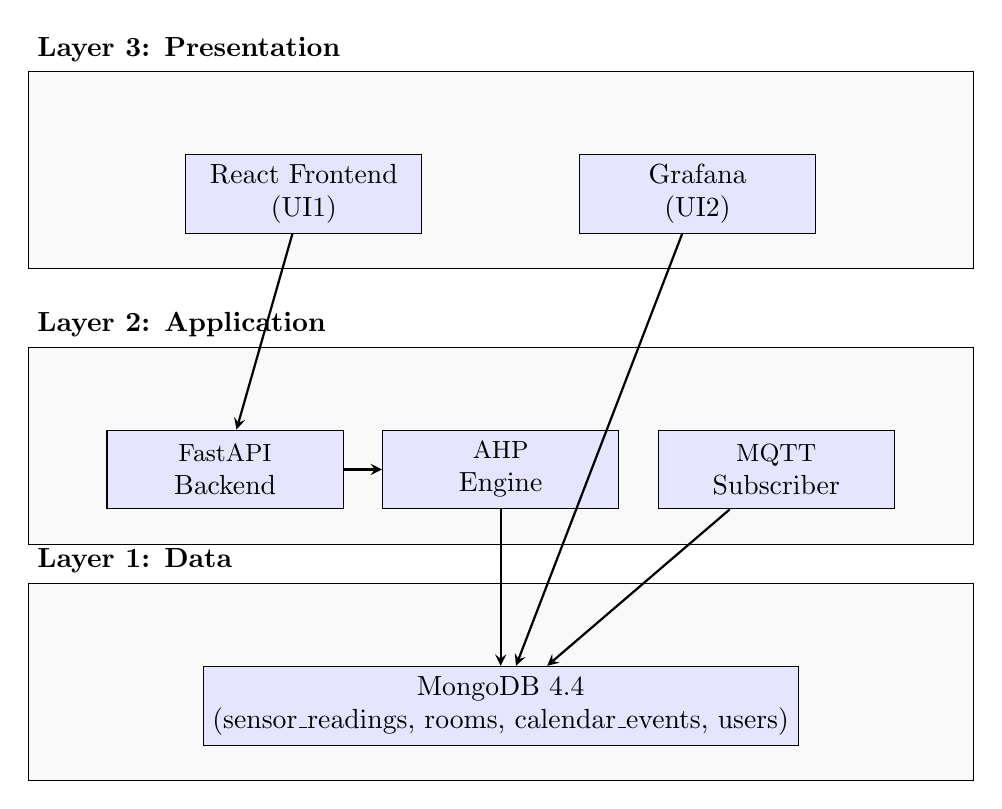
\begin{tikzpicture}[
        box/.style={rectangle, draw, minimum width=3cm, minimum height=1cm, align=center, fill=blue!10},
        layer/.style={rectangle, draw, minimum width=12cm, minimum height=2.5cm, align=center, fill=gray!5},
        arrow/.style={->, >=stealth, thick}
    ]

    % Layer 3 - Presentation
    \node[layer] (layer3) at (0,0) {};
    \node[above right] at (layer3.north west) {\textbf{Layer 3: Presentation}};
    \node[box] (react) at (-2.5,-0.3) {React Frontend\\(UI1)};
    \node[box] (grafana) at (2.5,-0.3) {Grafana\\(UI2)};

    % Layer 2 - Application
    \node[layer] (layer2) at (0,-3.5) {};
    \node[above right] at (layer2.north west) {\textbf{Layer 2: Application}};
    \node[box] (fastapi) at (-3.5,-3.8) {\small FastAPI\\Backend};
    \node[box] (ahp) at (0,-3.8) {\small AHP\\Engine};
    \node[box] (mqtt) at (3.5,-3.8) {\small MQTT\\Subscriber};

    % Layer 1 - Data
    \node[layer] (layer1) at (0,-6.5) {};
    \node[above right] at (layer1.north west) {\textbf{Layer 1: Data}};
    \node[box, minimum width=6cm] (mongodb) at (0,-6.8) {MongoDB 4.4\\(sensor\_readings, rooms, calendar\_events, users)};

    % Arrows
    \draw[arrow] (react) -- (fastapi);
    \draw[arrow] (grafana) -- (mongodb);
    \draw[arrow] (fastapi) -- (ahp);
    \draw[arrow] (ahp) -- (mongodb);
    \draw[arrow] (mqtt) -- (mongodb);

    \end{tikzpicture}
    \caption{Three-tier system architecture}
    \label{fig:architecture}
\end{figure}

% ============================================================
\section{Communication Protocols}
\label{sec:comm}
% ============================================================

The project specification required four communication layers (Comm~A through~D). Our implementation maps them as follows:

\begin{table}[H]
\centering
\small
\begin{tabular}{@{}p{1.5cm}p{3cm}p{2.8cm}p{5.5cm}@{}}
\toprule
\textbf{Layer} & \textbf{Protocol} & \textbf{Direction} & \textbf{Justification} \\
\midrule
Comm A & I\textsuperscript{2}C / Analog & Sensor $\to$ MCU & Low-power, short-range bus for reading environmental sensors \\
Comm B & MQTT & MCU $\to$ Broker & Lightweight pub/sub ideal for constrained IoT devices \\
Comm C & HTTP REST & Broker $\to$ DB & Reliable ingestion into MongoDB via FastAPI endpoints \\
Comm D & HTTP REST & Client $\to$ API & Standard web API consumed by React frontend and Grafana \\
\bottomrule
\end{tabular}
\caption{Communication protocol mapping}
\label{tab:comm}
\end{table}

\textbf{Why MQTT for Comm~B:} MQTT's publish/subscribe model decouples sensor nodes from the backend. It uses minimal bandwidth (important for constrained MCUs), supports QoS levels for delivery guarantees, and is the de facto standard for IoT telemetry.

\textbf{Why HTTP REST for Comm~C/D:} REST is a standard stateless protocol. Using HTTP for both ingestion and client access simplifies the stack and allows automatic Swagger documentation via FastAPI.

% ============================================================
\section{Database Design}
% ============================================================

\subsection{Why MongoDB}

We chose MongoDB for several reasons:
\begin{itemize}
    \item \textbf{Schema flexibility}: Sensor readings vary by type (temperature has different fields than air quality). A document model accommodates this without schema migrations.
    \item \textbf{Time-series affinity}: MongoDB's document structure maps naturally to timestamped sensor readings, and compound indexes on \texttt{(room\_name, sensor\_type, timestamp)} enable efficient range queries.
    \item \textbf{Async driver}: The Motor async driver integrates natively with FastAPI's async request handling, avoiding thread-pool overhead.
\end{itemize}

\subsection{Collections and Indexing}

\begin{table}[H]
\centering
\begin{tabular}{@{}lll@{}}
\toprule
\textbf{Collection} & \textbf{Purpose} & \textbf{Key Indexes} \\
\midrule
\texttt{sensor\_readings} & Time-series environmental data & \texttt{(room\_name, sensor\_type, timestamp)} \\
\texttt{rooms}            & Room metadata and facilities   & \texttt{(name)} unique \\
\texttt{calendar\_events} & Room bookings / availability   & \texttt{(room\_name, start\_time, end\_time)} \\
\texttt{users}            & Authentication accounts        & \texttt{(username)} unique \\
\bottomrule
\end{tabular}
\caption{MongoDB collections and primary indexes}
\label{tab:collections}
\end{table}

Indexes are created programmatically on application startup in \texttt{database.py}, ensuring they exist regardless of deployment method.

% ============================================================
\section{Decision Criteria: EU EN~16798-1}
% ============================================================

Room ranking is grounded in the European standard EN~16798-1 for indoor environmental quality. We selected \textbf{Category~II} thresholds (normal level of expectation for new and renovated buildings), which define optimal and acceptable ranges for each parameter:

\begin{table}[H]
\centering
\small
\begin{tabular}{@{}p{2.5cm}p{3cm}p{3cm}p{3.5cm}@{}}
\toprule
\textbf{Parameter} & \textbf{Optimal Range} & \textbf{Acceptable Range} & \textbf{Standard} \\
\midrule
Temperature   & 20--24\,\textdegree C & 18--26\,\textdegree C & EN 16798-1 \\
CO\textsubscript{2}  & $\leq$\,800\,ppm  & $\leq$\,1000\,ppm & EN 16798-1 \\
Humidity      & 40--60\,\%     & 30--70\,\%     & EN 16798-1 \\
Noise         & $<$\,35\,dBA   & $<$\,45\,dBA   & WHO Guidelines \\
Lighting      & 300--500\,lux  & 200--750\,lux  & EN 12464-1 \\
VOC           & $<$\,200\,ppb  & $<$\,400\,ppb  & WELL Standard \\
PM\textsubscript{2.5}   & $<$\,10\,\textmu g/m\textsuperscript{3}  & $<$\,25\,\textmu g/m\textsuperscript{3}  & WHO Guidelines \\
PM\textsubscript{10}    & $<$\,20\,\textmu g/m\textsuperscript{3}  & $<$\,50\,\textmu g/m\textsuperscript{3}  & WHO Guidelines \\
\bottomrule
\end{tabular}
\caption{Environmental thresholds used for score mapping}
\label{tab:eu_standards}
\end{table}

Each raw sensor value is normalized to a $[0, 1]$ score using piecewise linear mapping functions (implemented in \texttt{score\_mapping.py}). Values within the optimal range receive a score of~1.0; values outside the acceptable range receive~0.0; intermediate values are linearly interpolated.

\textbf{Note on facility scoring:} Room facilities (seating, equipment, A/V) are not binary filters but contribute scores to the Usability criterion. Rooms with capacity significantly exceeding requirements receive minor penalties to discourage resource waste, while rooms meeting exact requirements receive optimal scores.

\textbf{Occupancy Criterion (Bonus):} Beyond the six core environmental criteria, the production system can also use room occupancy detection via Vision AI V2 modules (Section~\ref{sec:hardware}). The \texttt{map\_occupancy()} function in Section~\ref{sec:hardware} scores lower occupancy higher, favoring rooms conducive to focused individual work over crowded collaborative spaces.

% ============================================================
\section{AHP Algorithm}
% ============================================================

\subsection{Why AHP}

The Analytic Hierarchy Process (Saaty, 1980) was chosen because:
\begin{itemize}
    \item It handles \textbf{multi-criteria} decisions with both quantitative (sensor data) and qualitative (user preferences) inputs.
    \item The \textbf{pairwise comparison} approach is intuitive for users - they compare criteria two at a time on a 1--9 scale rather than assigning abstract weights.
    \item Built-in \textbf{consistency checking} (CR~$< 0.1$) ensures that user preferences are logically coherent.
\end{itemize}

\subsection{Three-Level Hierarchy}

Our AHP model uses a three-level criteria hierarchy:

\begin{enumerate}
    \item \textbf{Level 1 -- Main Criteria}: Comfort, Health, Usability
    \item \textbf{Level 2 -- Sub-Criteria}:
    \begin{itemize}
        \item Comfort $\to$ Temperature, Lighting, Noise, Humidity
        \item Health $\to$ CO\textsubscript{2}, Air Quality (AQI), VOC, PM\textsubscript{2.5}, PM\textsubscript{10}
        \item Usability $\to$ Seating Capacity, Equipment, AV Facilities
    \end{itemize}
    \item \textbf{Level 3 -- Alternatives}: The candidate rooms (system evaluates 5 rooms in the prototype)
\end{enumerate}

\subsection{Implementation}

The AHP engine is modular, split across five files in \texttt{backend/app/ahp/}:

\begin{description}
    \item[\texttt{pairwise\_matrix.py}] Constructs and validates Saaty-scale pairwise comparison matrices. Enforces reciprocality ($a_{ji} = 1/a_{ij}$) and diagonal unity.
    \item[\texttt{eigenvector.py}] Computes priority weight vectors using the principal eigenvector method. Also provides geometric mean and normalized sum as alternatives. Calculates the Consistency Ratio:
    \[
        CR = \frac{CI}{RI}, \quad CI = \frac{\lambda_{\max} - n}{n - 1}
    \]
    where $RI$ is the Random Index for matrix size $n$.
    \item[\texttt{score\_mapping.py}] Normalizes raw sensor readings to $[0, 1]$ scores based on EU standard thresholds (Section~6). Implements mappings for all environmental sensors (temperature, CO\textsubscript{2}, humidity, VOC, PM\textsubscript{2.5}, PM\textsubscript{10}, light, noise) and facility criteria (seating capacity, equipment, A/V facilities). Rooms exceeding capacity by more than 50\% receive minor score reductions.
    \item[\texttt{aggregation.py}] Combines weighted scores using a hybrid method: 70\% Weighted Sum Model + 30\% Weighted Product Model. This balances compensatory and non-compensatory ranking behavior.
    \item[\texttt{ahp\_engine.py}] Runs the full pipeline: loads user preferences, builds pairwise matrices, extracts weights, maps sensor data to scores, aggregates, and returns ranked rooms.
\end{description}

\subsection{Consistency Checking}

Every pairwise matrix submitted by users is validated against the standard AHP consistency threshold ($CR < 0.1$). If preferences are inconsistent, the system uses default expert-defined matrices as fallback, ensuring the ranking always produces meaningful results.

% ============================================================
\section{Hardware Architecture \& Deployment}
\label{sec:hardware}
% ============================================================

Each monitored room has a physical sensor node that collects environmental and occupancy data. Arduino-based nodes read sensors and publish readings over MQTT to a central Raspberry Pi, which hosts the MQTT broker, MongoDB, and FastAPI backend.

\subsection{Platform Selection}

\begin{table}[H]
\centering
\small
\begin{tabular}{@{}p{2.5cm}p{4cm}p{6cm}@{}}
\toprule
\textbf{Component} & \textbf{Model/Specification} & \textbf{Purpose} \\
\midrule
Coordinator & Raspberry Pi 4 Model B (4GB RAM) & MQTT broker host, Docker orchestration, backend services \\
Sensor Node & Arduino Uno R3 + Ethernet Shield 2 (W5500) & Environmental data acquisition \& publishing \\
Occupancy Detection & Vision AI V2 & Computer vision person counting \\
Network Fabric & Ethernet (Cat5e/Cat6 wired) & Sensor node $\to$ coordinator connectivity \\
\bottomrule
\end{tabular}
\caption{Platform components}
\label{tab:platform}
\end{table}

All hardware components (Raspberry Pi~4, Arduino Uno, Ethernet Shield~2, Vision AI V2, and the sensor kit) were provided by the professor as the standard platform for this course.

\subsection{Sensor Specifications \& Wiring}

Each sensor node monitors six environmental parameters aligned with EN~16798-1 standards (Section~6) plus local status feedback. The Arduino firmware samples sensors at intervals optimized for response time versus MQTT message frequency, publishing aggregated readings as JSON payloads.

\begin{table}[H]
\centering
\small
\begin{tabular}{@{}p{2.2cm}p{2.2cm}p{1.8cm}p{2.2cm}p{1.5cm}p{2.2cm}@{}}
\toprule
\textbf{Sensor Type} & \textbf{Model/ Interface} & \textbf{Arduino Pin} & \textbf{Range} & \textbf{Sampling} & \textbf{AHP Criterion} \\
\midrule
Temperature/ Humidity & DHT11 Digital & GPIO D2 & 0 to 50\textdegree C, 20-90\% RH & Every 5s & Comfort (thermal, hygroscopic) \\
Sound Level & Analog Microphone & Analog A0 & 30-130 dB & Every 100ms & Comfort (acoustic) \\
Light Intensity & Photoresistor LDR & Analog A1 & 0-1000 lux & Every 500ms & Comfort (visual, EN 12464-1) \\
Air Quality & Grove Air Quality Sensor v1.3 & Analog A3 & 0-500 AQI & Every 5s & Health (air quality) \\
Status Display & Grove LCD RGB Backlight & I\textsuperscript{2}C (auto-detect 0x62) & 16$\times$2 characters & Event-driven & Local debugging feedback \\
Connectivity Status & Green LED & GPIO D4 & Binary on/off & Continuous & MQTT connection / air quality indicator \\
\bottomrule
\end{tabular}
\caption{Sensor pinout and specifications}
\label{tab:sensors}
\end{table}

Communication protocols (I\textsuperscript{2}C for LCD, MQTT for telemetry) are detailed in Section~\ref{sec:comm}. The Arduino firmware implements the Comm~A (sensor $\to$ MCU analog/digital) and Comm~B (MCU $\to$ broker MQTT) layers defined in Table~\ref{tab:comm}.

\textbf{Wiring Notes:} The Grove Base Shield v2 stacks on top of the Ethernet Shield 2, providing convenient 4-pin connectors for all sensors. The DHT11 connects via the D2 Grove connector (white 4-pin cable), analog sensors use yellow 4-pin cables on A0, A1, and A3, and the LCD uses the I\textsuperscript{2}C Grove connector. The Ethernet Shield occupies SPI bus pins D10-D13, leaving sufficient GPIO and analog pins for the sensor array.

\textbf{Wiring Diagram:}

\begin{lstlisting}[basicstyle=\small\ttfamily]
+-------------------------------------------------------------+
|                    ARDUINO UNO R3                           |
|  +-----------------------------------------------------+    |
|  |              ETHERNET SHIELD 2                      |    |
|  |  +-----------------------------------------------+  |    |
|  |  |            GROVE BASE SHIELD v2               |  |    |
|  |  |                                               |  |    |
|  |  |  [D2]  <- Temp&Humidity (white 4-pin cable)   |  |    |
|  |  |  [D4]  <- Green LED                           |  |    |
|  |  |                                               |  |    |
|  |  |  [A0]  <- Sound Sensor (yellow 4-pin cable)   |  |    |
|  |  |  [A1]  <- Light Sensor (yellow 4-pin cable)   |  |    |
|  |  |  [A3]  <- Air Quality (yellow 4-pin cable)    |  |    |
|  |  |                                               |  |    |
|  |  |  [I2C] <- LCD RGB Backlight (4-pin cable)     |  |    |
|  |  +-----------------------------------------------+  |    |
|  |                                                     |    |
|  |  [RJ45] -----> Router/Switch (same network as Pi)   |    |
|  +-----------------------------------------------------+    |
|                                                             |
|  [USB] -----> Computer (for programming/power)              |
|  [DC Jack] -> 9V power supply (alternative)                 |
+-------------------------------------------------------------+
\end{lstlisting}

\subsection{Vision AI Integration for Occupancy Detection}

In addition to environmental sensors, we use Vision AI V2 modules for occupancy detection, which adds a seventh criterion to the AHP algorithm. Vision-based person counting is more accurate than PIR motion sensors, and the \texttt{map\_occupancy()} scoring function (Section~7) to penalize overcrowded rooms in ranking results.

\textbf{UART Connection:}

\begin{lstlisting}[basicstyle=\small\ttfamily]
Vision AI V2 -> Raspberry Pi 4 GPIO Header
-----------------------------------------
TX (White) -> GPIO 15 (Pin 10) - RXD
RX (Green) -> GPIO 14 (Pin 8)  - TXD
GND (Black) -> GND (Pin 6)
VCC (Red)  -> 3.3V (Pin 1) - Max 50mA draw

Configuration: 115200 baud, 8N1
(8 data bits, no parity, 1 stop bit)
\end{lstlisting}

\textbf{Data Flow:} The Vision AI module processes video frames locally using a pre-trained person detection model, outputting integer person counts over UART at 1Hz. A Python daemon script (\texttt{vision\_ai\_reader.py}) running on the Raspberry Pi reads the serial stream via \texttt{/dev/ttyAMA0} and publishes counts to MQTT topic \texttt{iot/\{ROOM\_NAME\}/occupancy}. The MQTT subscriber service writes occupancy readings to the same \texttt{sensor\_readings} MongoDB collection with \texttt{sensor\_type: 'occupancy'} and \texttt{unit: 'count'}.

\textbf{Scoring Integration:} The backend's AHP implementation includes \texttt{OCCUPANCY\_CONFIG} in \texttt{score\_mapping.py}, which scores lower occupancy higher (empty room = 1.0, overcapacity = 0.0-0.2). This favors emptier rooms for focused work and penalizes crowded ones.

\subsection{Data Collection Architecture}

The firmware-to-database pipeline uses MQTT's publish-subscribe model, so sensor nodes don't need to know about the backend. Each Arduino publishes JSON-formatted sensor readings to room-specific topics -- adding more rooms just means adding more publishers.

\begin{lstlisting}[basicstyle=\small\ttfamily]
+-----------------------------------------------------+
| Arduino Firmware (room_sensors.ino)                |
|  * Polls sensors at configured intervals           |
|  * Converts analog readings to physical units      |
|  * Constructs JSON: {"temperature": 23.5, ...}     |
|  * Publishes to: iot/{ROOM_NAME}/sensors           |
+------------------------------+----------------------+
                               | MQTT over Ethernet
                               v
+-----------------------------------------------------+
| Mosquitto MQTT Broker (Raspberry Pi)               |
|  * Port 1883 (unencrypted, local network only)     |
|  * Topic wildcards: iot/+/sensors, iot/+/occupancy |
+------------------------------+----------------------+
                               | Topic subscription
                               v
+-----------------------------------------------------+
| Python Bridge (mqtt_subscriber.py)                 |
|  * paho-mqtt client subscribes to iot/#            |
|  * Parses JSON, validates data types               |
|  * Adds timestamp, writes to MongoDB               |
+------------------------------+----------------------+
                               | PyMongo async write
                               v
+-----------------------------------------------------+
| MongoDB Collection: sensor_readings                |
|  * Document schema: {room_name, sensor_type,       |
|    value, unit, timestamp, ...}                    |
+-----------------------------------------------------+
\end{lstlisting}

\textbf{Sample MQTT Payload:}

\begin{lstlisting}[basicstyle=\small\ttfamily]
{
  "temperature": 23.5,
  "humidity": 55,
  "sound": 42,
  "light_intensity": 450,
  "air_quality": 35
}
\end{lstlisting}

\textbf{Production Deployment:} Both \texttt{mqtt\_subscriber.py} and \texttt{vision\_ai\_reader.py} deploy as systemd services (\texttt{mqtt\_subscriber.service}, \texttt{vision\_ai.service}) on the Raspberry Pi, configured for automatic startup on boot. Services implement graceful signal handling (SIGTERM/SIGINT) for clean shutdown and MQTT disconnection, preventing message loss during restarts.

\subsection{Power \& Deployment Considerations}

\begin{table}[H]
\centering
\small
\begin{tabular}{@{}p{3cm}p{1.5cm}p{2.2cm}p{2.8cm}p{3cm}@{}}
\toprule
\textbf{Component} & \textbf{Voltage} & \textbf{Current Draw} & \textbf{Power Supply} & \textbf{Notes} \\
\midrule
Arduino Uno + Ethernet Shield & 5V DC & 200-500mA (avg) & USB or 7-12V barrel jack & Peaks during Ethernet TX \\
Raspberry Pi 4 (4GB) & 5V DC & 600-1200mA (avg) & USB-C (5V/3A recommended) & Peaks during Docker container startup \\
Vision AI V2 & 3.3V DC & $<$50mA & Pi GPIO header (Pin 1) & Powered directly by Pi \\
DHT11 + Analog Sensors & 3.3-5V DC & $<$20mA total & Arduino 5V rail & Negligible power draw \\
\bottomrule
\end{tabular}
\caption{Power requirements}
\label{tab:power}
\end{table}

\textbf{Physical Installation:} Sensor nodes mount in standard electrical junction boxes (single-gang) near room entrances, with Ethernet cable routed through conduit to centralized network switch. The Raspberry Pi coordinator resides in a server room or network closet alongside the Ethernet switch, minimizing cable runs. Vision AI modules mount at doorway height (1.5-2m) for optimal people counting accuracy.

\textbf{Scalability Analysis:} The current prototype instruments 5 rooms (Room\_1 through Room\_5) with a Bill of Materials cost of approximately \$40 USD per room (Arduino \$25, Ethernet Shield \$10, sensors \$5 total). The Mosquitto MQTT broker on Raspberry Pi~4 can handle many concurrent MQTT clients efficiently, so the system can scale to full building floors (20-50 rooms) without hardware changes. Vertical scaling to multiple buildings requires additional Raspberry Pi coordinators, each operating an independent MQTT broker with backend API endpoints federated via DNS load balancing.

% ============================================================
\section{REST API Design}
% ============================================================

\subsection{Why FastAPI}

\begin{itemize}
    \item \textbf{Automatic OpenAPI/Swagger}: Every endpoint is self-documented with request/response schemas, satisfying the Swagger documentation requirement with zero extra effort.
    \item \textbf{Async-native}: Built on Starlette/ASGI, it handles concurrent sensor queries without blocking.
    \item \textbf{Pydantic validation}: Request bodies are validated against typed models at the framework level, meaning less repetitive code.
    \item \textbf{Lightweight}: Suitable for deployment on a Raspberry Pi~4.
\end{itemize}

\subsection{Endpoint Structure}

All endpoints are versioned under \texttt{/api/v1/}:

\begin{table}[H]
\centering
\small
\begin{tabular}{@{}p{1.3cm}p{6.5cm}p{5cm}@{}}
\toprule
\textbf{Method} & \textbf{Endpoint} & \textbf{Purpose} \\
\midrule
POST & \texttt{/api/v1/rank} & Room ranking (main DSS endpoint) \\
GET  & \texttt{/api/v1/rooms/} & List rooms with facilities \\
GET  & \texttt{/api/v1/sensors/\{room\}/\{type\}} & Sensor readings (time range) \\
GET  & \texttt{/api/v1/sensors/\{room\}/latest} & Latest sensor snapshot \\
GET  & \texttt{/api/v1/calendar/availability/\{room\}} & Room availability \\
POST & \texttt{/api/v1/auth/login} & JWT authentication \\
POST & \texttt{/api/v1/auth/register} & User registration \\
GET  & \texttt{/health} & Health check (DB connectivity) \\
\bottomrule
\end{tabular}
\caption{REST API endpoints}
\label{tab:endpoints}
\end{table}

\begin{figure}[H]
    \centering
    \includegraphics[width=\textwidth]{swagger_ui.png}
    \caption{Swagger UI showing API documentation}
    \label{fig:swagger}
\end{figure}

% ============================================================
\section{Frontend -- End-User Interface (UI1)}
% ============================================================

\subsection{Technology Choices}

\begin{itemize}
    \item \textbf{React~19 + Vite~7}: Vite provides sub-second hot module replacement during development and optimized production builds. React's component model maps cleanly to our UI structure (preference input, ranking display, score breakdown).
    \item \textbf{Tailwind~CSS}: Utility-first styling avoids context-switching between component logic and separate stylesheets.
    \item \textbf{Recharts}: Declarative charting library for visualizing score breakdowns.
    \item \textbf{Mock API fallback}: Setting \texttt{VITE\_USE\_MOCK\_API=true} enables fully offline frontend development, decoupling UI work from backend availability.
\end{itemize}

\subsection{User Flow}

\begin{enumerate}
    \item User navigates to the room selection page (\texttt{/select-room}).
    \item The \texttt{PreferenceMatrix} component presents Saaty-scale sliders for pairwise comparisons between criteria (comfort, health, usability).
    \item The \texttt{ProfileAdjuster} allows optional threshold overrides (e.g.\ minimum temperature).
    \item On submission, preferences are transformed to backend format by \texttt{apiClient.js} and sent to \texttt{POST /api/v1/rank}.
    \item Results are displayed via \texttt{RoomRanking} (ordered list) and \texttt{ScoreBreakdown} (per-criterion charts).
\end{enumerate}

\begin{figure}[H]
    \centering
    \includegraphics[width=\textwidth]{ui_room_selection.png}
    \caption{Room selection interface with preference input}
    \label{fig:ui1}
\end{figure}

% ============================================================
\section{Admin Dashboard (UI2) -- Grafana}
% ============================================================

We chose Grafana for the admin monitoring dashboard because:
\begin{itemize}
    \item It connects natively to MongoDB via plugins, requiring no custom dashboard code.
    \item It provides real-time auto-refreshing panels for sensor time-series data.
    \item Pre-built visualization types (gauges, time-series graphs, heatmaps) cover all monitoring needs.
    \item Alerting rules can be configured for threshold violations (e.g.\ CO\textsubscript{2} exceeding 1000\,ppm).
\end{itemize}

Dashboard configurations are versioned in the \texttt{grafana/} directory and provisioned automatically via Docker Compose. The dashboard is accessible at \texttt{http://localhost:3000}.

\begin{figure}[H]
    \centering
    \includegraphics[width=\textwidth]{grafana_dashboard.png}
    \caption{Grafana admin dashboard showing real-time sensor data}
    \label{fig:grafana}
\end{figure}

% ============================================================
\section{Authentication (Bonus)}
% ============================================================

We implemented JWT-based authentication as a bonus feature:

\begin{itemize}
    \item \textbf{Algorithm}: HS256 with a server-side secret key.
    \item \textbf{Token lifetime}: 30 minutes (configurable via \texttt{ACCESS\_TOKEN\_EXPIRE\_MINUTES}).
    \item \textbf{Password storage}: Bcrypt hashing with automatic salt generation.
    \item \textbf{Frontend integration}: Tokens are stored in \texttt{localStorage} and attached to requests via an Axios interceptor.
    \item \textbf{Password policy}: Minimum 8 characters, at least one uppercase letter, one lowercase letter, and one digit.
\end{itemize}

This secures the ranking endpoint and and would let us save per-user preferences in the future.

% ============================================================
\section{Containerization and Deployment}
% ============================================================

\subsection{Docker Compose Architecture}

All services are defined in a single \texttt{docker-compose.yml}:

\begin{table}[H]
\centering
\begin{tabular}{@{}llll@{}}
\toprule
\textbf{Service} & \textbf{Image} & \textbf{Port} & \textbf{Notes} \\
\midrule
\texttt{mongodb}       & mongo:4.4              & 27017 & Persistent volume, health check \\
\texttt{backend}       & Custom (Python 3.11)   & 8000  & Waits for MongoDB health \\
\texttt{mongo-express} & mongo-express:latest   & 8081  & Dev profile only \\
\bottomrule
\end{tabular}
\caption{Docker Compose services}
\label{tab:docker}
\end{table}

\textbf{Design decisions}:
\begin{itemize}
    \item Services communicate over a private \texttt{iot-network} bridge, isolating traffic from the host.
    \item The backend uses \texttt{depends\_on} with a health check condition, ensuring MongoDB is ready before accepting requests.
    \item The backend Dockerfile uses a multi-stage build optimized for ARM (Raspberry Pi~4 deployment) and runs as a non-root user for security.
    \item Mongo Express is gated behind a \texttt{dev} profile (\texttt{docker-compose --profile dev up}) to avoid exposing it in production.
\end{itemize}

% ============================================================
\section{Testing}
% ============================================================

\subsection{AHP Unit Tests}

The \texttt{unit/} directory contains five test modules covering each AHP component:

\begin{itemize}
    \item \texttt{test\_pairwise\_matrix.py} -- Matrix construction, reciprocality, validation
    \item \texttt{test\_eigenvector.py} -- Weight extraction, consistency ratio calculation
    \item \texttt{test\_score\_mapping.py} -- Sensor value normalization against EU thresholds
    \item \texttt{test\_aggregation.py} -- WSM, WPM, and combined aggregation
    \item \texttt{test\_ahp\_engine.py} -- End-to-end ranking pipeline
\end{itemize}

\subsection{Backend Integration Tests}

The \texttt{backend/tests/} directory contains API-level tests using \texttt{pytest} and \texttt{httpx}, covering JWT authentication flows and endpoint response validation.

% ============================================================
\section{Conclusion}
% ============================================================

Our IoT Room Selection DSS covers all eight project requirements with a straightforward design: sensor data flows through standardized communication protocols into MongoDB, the AHP algorithm produces clear rankings grounded in EU standards, and two distinct interfaces serve end users and administrators. Docker containerization ensures reproducible deployment across development machines and the target Raspberry Pi hardware.

\end{document}
